% Revisão OK 25/09
\chapter{Sistemas Similares}
Os EFBs possuem funções variadas como cálculo de combustível, gasto de combustível
em voo, velocidades de decolagem, etc. \cite{wired-efb} Para aeronaves mais novas, como o Airbus 
A320neo (New Engine Option), é difícil implementar o cálculo de performance e combustível, pois não 
é disponibilizado ao público como este cálculo é feito. Ferramentas encontradas 
na Internet \cite{a320-perf}, normalmente usan engenharia reversa, e, portanto, 
podem apresentar resultados diferentes de um cálculo oficial feito no aplicativo
de tablet.

Nos simuladores de voo para computador pessoal, algumas aeronaves simulam
este equipamento como o Airbus A320neo desenvolvido pela \textit{FlyByWire Simulations}. 
Apesar de ser uma aeronave \textit{freeware}, ela é bem sofisticada, chegando ao 
nível de realismo da \textit{Fenix Simulations} ou da \textit{ToLiss Simulations}, 
duas produtoras com modelos pagos do A320.

\begin{figure}%
    \centering
    \subfloat[\centering EFB no Flight Simulator 2020 na aeronave A320neo]{{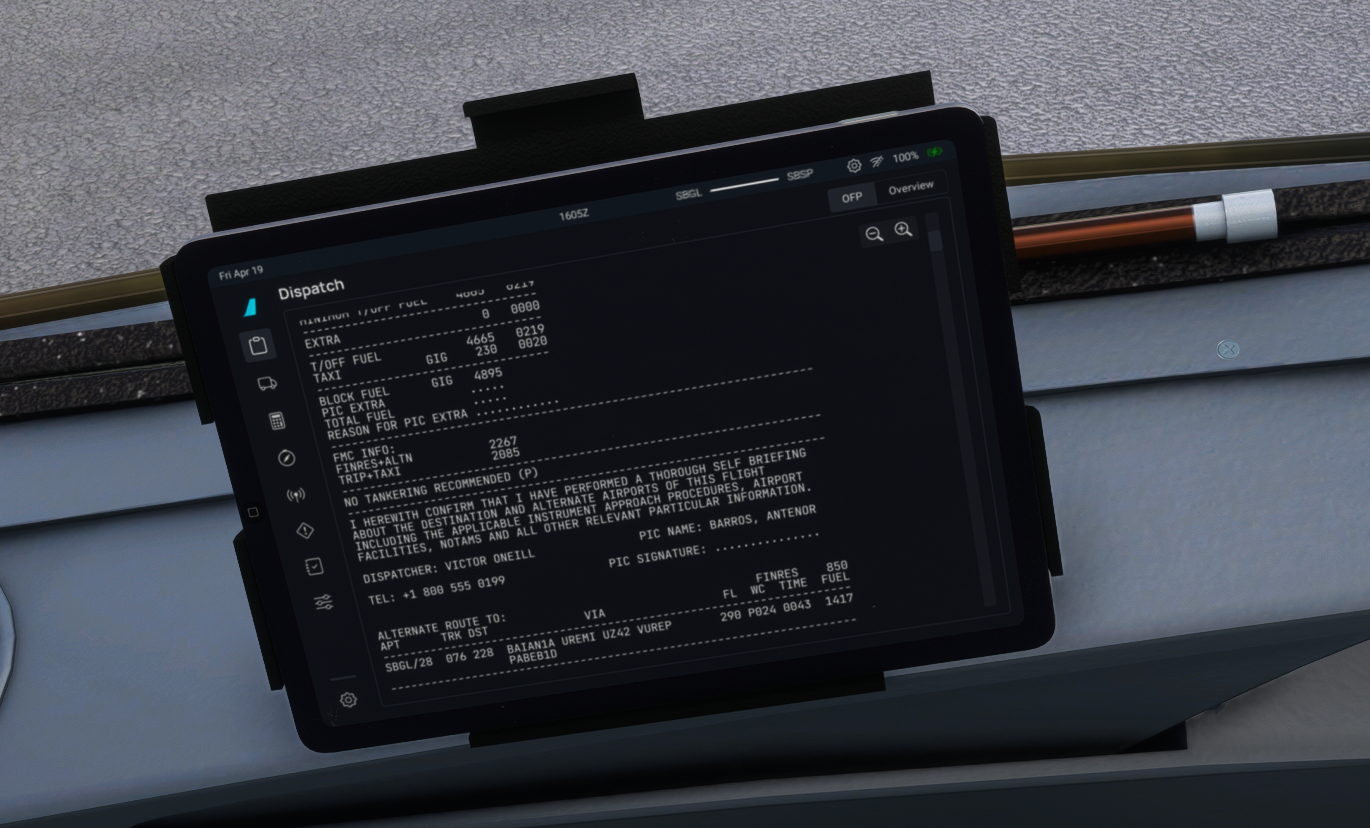
\includegraphics[width=0.47\linewidth]{img/efb-a320.png} }}%
    \qquad
    \subfloat[\centering EFB real \cite{wired-efb}]{{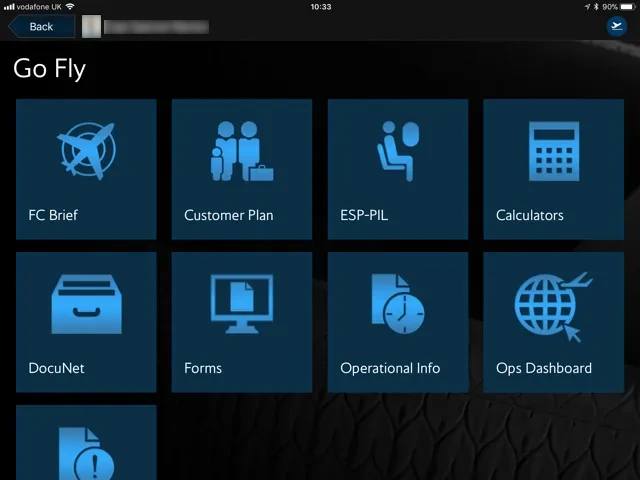
\includegraphics[width=0.45\linewidth]{img/real-flight-bag.png} }}%
    \caption{Exemplos de Electronic Flight Bag (EFB)}
    \label{fig:example}%
\end{figure}

Uma das informações importantes para a realização de um voo é o METAR. Trata-se 
de uma string codificada com as condições meteorológicas atuais de um aeródromo. 
Todos os pilotos aprendem a ler um METAR.

Contudo, o METAR do aeródromo não se encontra disponível no EFB. É possível usar
 o computador de bordo da aeronave (FMC) e conseguir esta informação. Também, é 
 possível sintonizar na frequência do ATIS, mas isto só funcionará se o avião
 estiver perto do aeródromo.

O que muitos usuários fazem é acessar o AISWEB 
(\url{https://aisweb.decea.mil.br/}), sistema oficial brasileiro de informações
aeronáuticas. 

\begin{figure}[ht]
    \begin{center}
    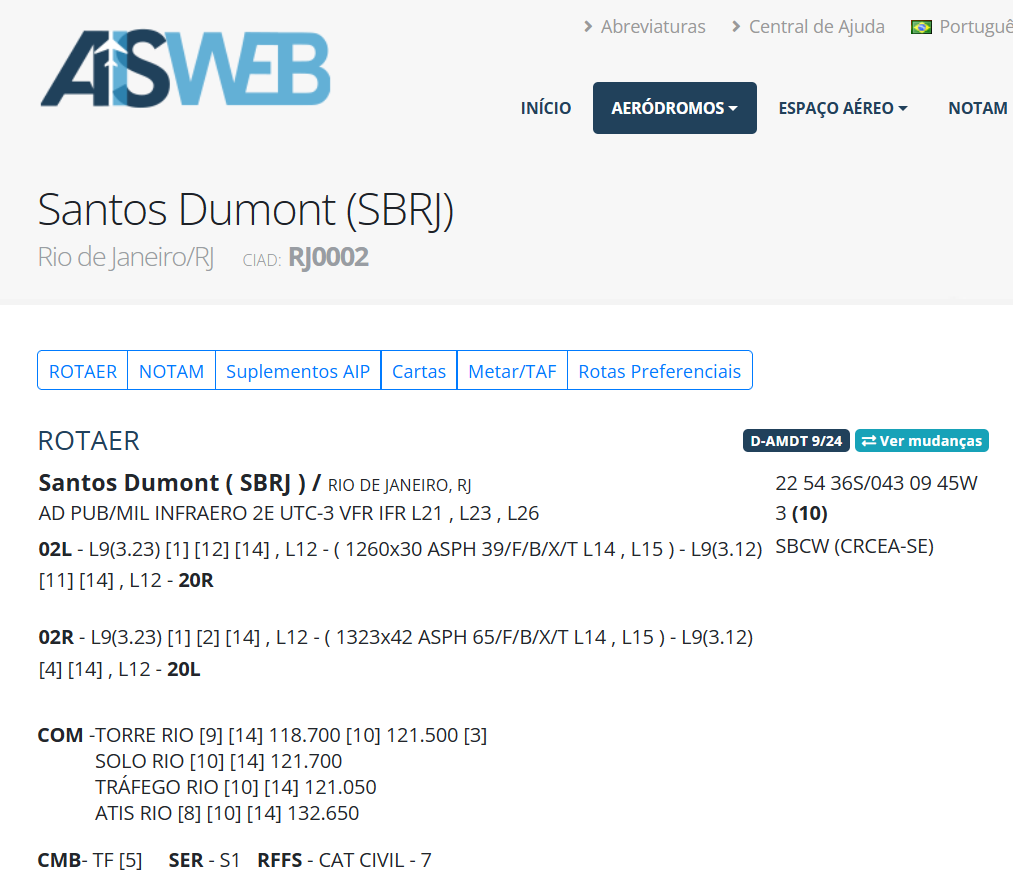
\includegraphics[width=350pt]{img/aisweb.png}
    \caption{AISWEB com informações de pista, frequências de comunicação e navegação para o Santos Dumont}
    \label{fig:aisweb}
    \end{center}
\end{figure}

É um site extremamente completo e usado em operações reais, mas para o usuário 
iniciante seria de valia uma interface mais simples. O AISWEB exibe o METAR no 
aeroporto, mas não explica para o que cada campo serve.

\begin{figure}[ht]
    \begin{center}
    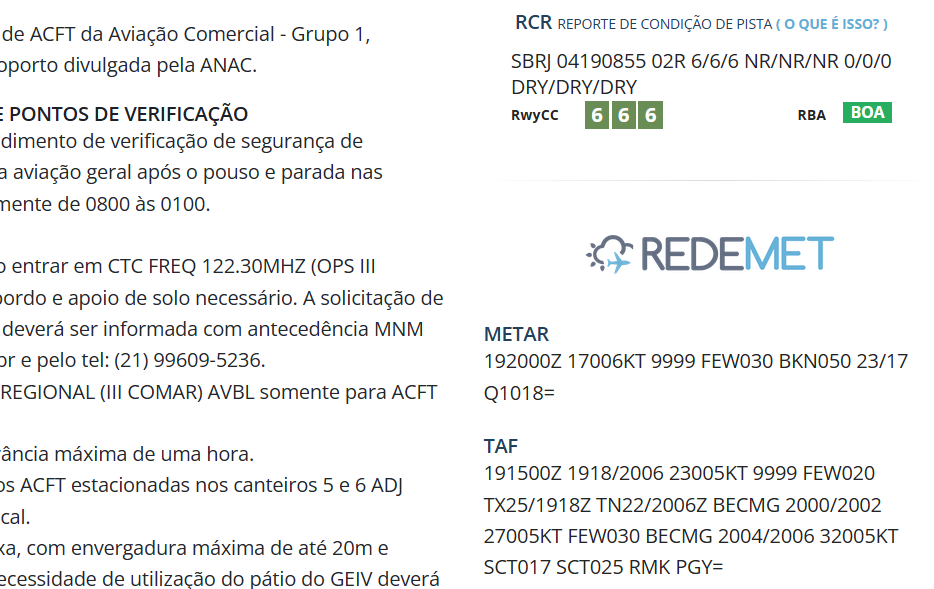
\includegraphics[width=200pt]{img/metar-aisweb.png}
    \caption{METAR do Santos Dumont no AISWEB}
    \label{fig:aisweb}
    \end{center}
\end{figure}

O site METAR-TAF (\url{https://metar-taf.com/}) é o \textit{decoder} mais conhecido. 
Possui
uma interface gráfica bem construída e muito fácil de entender, mas não possui a
lista de frequência dos aeroportos e de radionavegação. Como o nome deste sugere,
também é disponibilizado o TAF que é parecido com o METAR, mas o TAF é uma 
previsão das condições.

\begin{figure}[ht]
    \begin{center}
    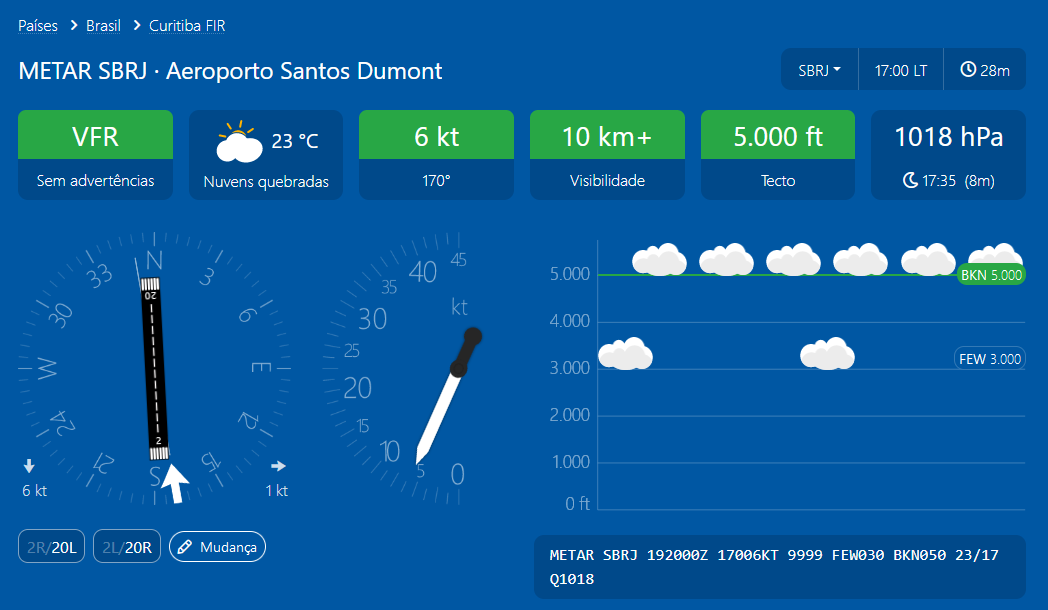
\includegraphics[width=400pt]{img/ui-metar-taf.png}
    \caption{Interface gráfica do METAR-TAF}
    \label{fig:metar-taf}
    \end{center}
\end{figure}
